\documentclass[a4paper]{article}

\usepackage[utf8]{inputenc}
\usepackage[portuges]{babel}
\usepackage{indentfirst}
\usepackage{graphicx}
\usepackage{float}
\usepackage{caption}
\usepackage{subcaption}
\usepackage[T1]{fontenc}
\usepackage{listings}
\usepackage{amsmath}
\usepackage{mathtools}
\renewcommand{\familydefault}{\sfdefault}


\title{Projeto de Computação Gráfica - Fase 2}
\author{Diogo Braga A82547 \and João Silva A82005 \and Ricardo Caçador A81064
\and Ricardo Veloso A81919}
\date{\today}

\begin{document}

\maketitle

\begin{abstract}
Neste relatório é apresentada a segunda fase dum projeto no qual a intenção é desenvolver um mecanismo baseado em gráficos 3D e fornecer exemplos de uso que mostrem o seu potencial. Este projeto é desenvolvido no âmbito da unidade curricular de Computação Gráfica.
\end{abstract}

\tableofcontents


\newpage

\section{Introdução}
\label{sec:intro}

!!!!!!!!!!!!!!!!!!!!!!!!!!!!!!!!!!!!!!!!! POR FAZER !!!!!!!!!!!!!!!!!!!!!!!!!!!!!!!!!!!!!!!!!

Esta primeira fase tem como objetivo a criação de duas aplicacões: \textit{generator} e \textit{engine}.

O \textit{generator} cria/reescreve um ficheiro (passado como parâmetro) que contém todos os vértices necessários para o desenho de uma determinada superfície, bem como o número de triângulos no início desse mesmo ficheiro.

No caso do \textit{engine} é necessário que este leia um ficheiro do tipo XML onde se encontra a referência para o ficheiro criado/reescrito, que queremos ler para depois ser gerada a figura pretendida.

De seguida, iremos apresentar todos os algoritmos e equações, bem como as suas respetivas explicações, que foram utilizados para a realização das duas aplicações. Também serão apresentadas figuras que contém código e figuras ilustrativas dos algoritmos/equações.

\section{Estrutura da Pasta do Projeto}
\label{sec:estrutura}

!!!!!!!!!!!!!!!!!!!!!!!!!!!!!!!!!!!!!!!!! POR FAZER !!!!!!!!!!!!!!!!!!!!!!!!!!!!!!!!!!!!!!!!!

Para um entendimento mais claro da estrutura do projeto, achamos por bem referenciar a estrutura da pasta do projeto.
O projeto entregue contêm para além do relatório, 4 pastas como é possível verificar na seguinte figura.

\begin{figure}[H]
\centering
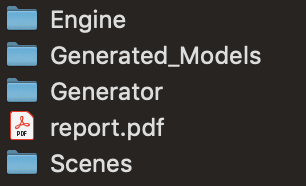
\includegraphics[scale=1.0]{estrutura.png}
\caption{Estrutura da pasta.}
\label{img:estrutura}
\end{figure}

Na pasta \textbf{Engine} residem os ficheiros relativos ao programa \emph{engine}, bem como ficheiros relativos à biblioteca \emph{tinyxml2}. Contém ainda um ficheiro de configuração \emph{cmake}.

Na pasta \textbf{Generator} residem os ficheiros relativos ao programa \emph{generator}. Contém ainda um ficheiro de configuração \emph{cmake}.

Na pasta \textbf{Generated\_Models} residem os ficheiros que contêm os pontos gerados para cada figura, criados pelo programa \emph{generator}.

Na pasta \textbf{Scenes} reside o ficheiro \emph{XML} que contém os nomes dos ficheiros que o programa \emph{engine} tem que carregar posteriormente.


\newpage

\section{Parser XML}
\label{sec:parser}

\subsection{Ficheiro}
\label{sec:ficheiro}

\subsection{Funcionamento}
\label{sec:funcionamento}


\newpage

\section{Estruturas de Dados}
\label{sec:estruturas}

\subsection{Tree}
\label{sec:tree}

\subsection{Figure}
\label{sec:figure}

\subsection{Color}
\label{sec:color}

\subsection{Scale}
\label{sec:scale}

\subsection{Rotation}
\label{sec:rotation}

\subsection{Translation}
\label{sec:translation}

\subsection{Point}
\label{sec:point}


\newpage

\section{\textit{Render Scene}}


\newpage

\section{Conclusão}
\label{sec:conclusao}

!!!!!!!!!!!!!!!!!!!!!!!!!!!!!!!!!!!!!!!!! POR FAZER !!!!!!!!!!!!!!!!!!!!!!!!!!!!!!!!!!!!!!!!!

Terminada a realização da fase 1 - primitivas gráficas, o grupo sente que realizou com sucesso  as 4 primitivas gráficas que compunham esta fase (plane, box, sphere e cone).  Assim, depois de uma revisão integral ao trabalho achamos que estamos preparados e num bom caminho para a realização de um bom projeto.
No geral não sentimos muitas dificuldades em nenhuma das primitivas gráficas pois também contamos com a ajuda da câmera que implementamos que permitiu uma melhor visualização do que estávamos a fazer bem ou mal.


\section{Bibliografia}
\label{sec:bibliografia}

!!!!!!!!!!!!!!!!!!!!!!!!!!!!!!!!!!!!!!!!! POR FAZER !!!!!!!!!!!!!!!!!!!!!!!!!!!!!!!!!!!!!!!!!

https://www.suapesquisa.com/astronomia/distancia\_sol\_planetas.htm

\end{document}
